% Options for packages loaded elsewhere
\PassOptionsToPackage{unicode}{hyperref}
\PassOptionsToPackage{hyphens}{url}
\PassOptionsToPackage{dvipsnames,svgnames,x11names}{xcolor}
%
\documentclass[
  letterpaper,
  DIV=11,
  numbers=noendperiod]{scrartcl}

\usepackage{amsmath,amssymb}
\usepackage{lmodern}
\usepackage{iftex}
\ifPDFTeX
  \usepackage[T1]{fontenc}
  \usepackage[utf8]{inputenc}
  \usepackage{textcomp} % provide euro and other symbols
\else % if luatex or xetex
  \usepackage{unicode-math}
  \defaultfontfeatures{Scale=MatchLowercase}
  \defaultfontfeatures[\rmfamily]{Ligatures=TeX,Scale=1}
\fi
% Use upquote if available, for straight quotes in verbatim environments
\IfFileExists{upquote.sty}{\usepackage{upquote}}{}
\IfFileExists{microtype.sty}{% use microtype if available
  \usepackage[]{microtype}
  \UseMicrotypeSet[protrusion]{basicmath} % disable protrusion for tt fonts
}{}
\makeatletter
\@ifundefined{KOMAClassName}{% if non-KOMA class
  \IfFileExists{parskip.sty}{%
    \usepackage{parskip}
  }{% else
    \setlength{\parindent}{0pt}
    \setlength{\parskip}{6pt plus 2pt minus 1pt}}
}{% if KOMA class
  \KOMAoptions{parskip=half}}
\makeatother
\usepackage{xcolor}
\setlength{\emergencystretch}{3em} % prevent overfull lines
\setcounter{secnumdepth}{-\maxdimen} % remove section numbering
% Make \paragraph and \subparagraph free-standing
\ifx\paragraph\undefined\else
  \let\oldparagraph\paragraph
  \renewcommand{\paragraph}[1]{\oldparagraph{#1}\mbox{}}
\fi
\ifx\subparagraph\undefined\else
  \let\oldsubparagraph\subparagraph
  \renewcommand{\subparagraph}[1]{\oldsubparagraph{#1}\mbox{}}
\fi


\providecommand{\tightlist}{%
  \setlength{\itemsep}{0pt}\setlength{\parskip}{0pt}}\usepackage{longtable,booktabs,array}
\usepackage{calc} % for calculating minipage widths
% Correct order of tables after \paragraph or \subparagraph
\usepackage{etoolbox}
\makeatletter
\patchcmd\longtable{\par}{\if@noskipsec\mbox{}\fi\par}{}{}
\makeatother
% Allow footnotes in longtable head/foot
\IfFileExists{footnotehyper.sty}{\usepackage{footnotehyper}}{\usepackage{footnote}}
\makesavenoteenv{longtable}
\usepackage{graphicx}
\makeatletter
\def\maxwidth{\ifdim\Gin@nat@width>\linewidth\linewidth\else\Gin@nat@width\fi}
\def\maxheight{\ifdim\Gin@nat@height>\textheight\textheight\else\Gin@nat@height\fi}
\makeatother
% Scale images if necessary, so that they will not overflow the page
% margins by default, and it is still possible to overwrite the defaults
% using explicit options in \includegraphics[width, height, ...]{}
\setkeys{Gin}{width=\maxwidth,height=\maxheight,keepaspectratio}
% Set default figure placement to htbp
\makeatletter
\def\fps@figure{htbp}
\makeatother

\KOMAoption{captions}{tableheading}
\makeatletter
\makeatother
\makeatletter
\makeatother
\makeatletter
\@ifpackageloaded{caption}{}{\usepackage{caption}}
\AtBeginDocument{%
\ifdefined\contentsname
  \renewcommand*\contentsname{Table of contents}
\else
  \newcommand\contentsname{Table of contents}
\fi
\ifdefined\listfigurename
  \renewcommand*\listfigurename{List of Figures}
\else
  \newcommand\listfigurename{List of Figures}
\fi
\ifdefined\listtablename
  \renewcommand*\listtablename{List of Tables}
\else
  \newcommand\listtablename{List of Tables}
\fi
\ifdefined\figurename
  \renewcommand*\figurename{Figure}
\else
  \newcommand\figurename{Figure}
\fi
\ifdefined\tablename
  \renewcommand*\tablename{Table}
\else
  \newcommand\tablename{Table}
\fi
}
\@ifpackageloaded{float}{}{\usepackage{float}}
\floatstyle{ruled}
\@ifundefined{c@chapter}{\newfloat{codelisting}{h}{lop}}{\newfloat{codelisting}{h}{lop}[chapter]}
\floatname{codelisting}{Listing}
\newcommand*\listoflistings{\listof{codelisting}{List of Listings}}
\makeatother
\makeatletter
\@ifpackageloaded{caption}{}{\usepackage{caption}}
\@ifpackageloaded{subcaption}{}{\usepackage{subcaption}}
\makeatother
\makeatletter
\@ifpackageloaded{tcolorbox}{}{\usepackage[many]{tcolorbox}}
\makeatother
\makeatletter
\@ifundefined{shadecolor}{\definecolor{shadecolor}{rgb}{.97, .97, .97}}
\makeatother
\makeatletter
\makeatother
\ifLuaTeX
  \usepackage{selnolig}  % disable illegal ligatures
\fi
\IfFileExists{bookmark.sty}{\usepackage{bookmark}}{\usepackage{hyperref}}
\IfFileExists{xurl.sty}{\usepackage{xurl}}{} % add URL line breaks if available
\urlstyle{same} % disable monospaced font for URLs
\hypersetup{
  colorlinks=true,
  linkcolor={blue},
  filecolor={Maroon},
  citecolor={Blue},
  urlcolor={blue},
  pdfcreator={LaTeX via pandoc}}

\author{}
\date{}

\begin{document}
\ifdefined\Shaded\renewenvironment{Shaded}{\begin{tcolorbox}[boxrule=0pt, breakable, enhanced, sharp corners, interior hidden, frame hidden, borderline west={3pt}{0pt}{shadecolor}]}{\end{tcolorbox}}\fi

Caleb Skinner

Global Health Survey Questions 11-15

\hypertarget{questions}{%
\subsection{Questions:}\label{questions}}

\hypertarget{in-your-opinion-what-are-the-greatest-barriers-to-providing-healthcare-in-low-resource-settings}{%
\subsection{11. In your opinion, what are the greatest barriers to
providing healthcare in low-resource
settings?}\label{in-your-opinion-what-are-the-greatest-barriers-to-providing-healthcare-in-low-resource-settings}}

A. Overall Results for Barriers to Providing Healthcare to Low-Resource
Settings

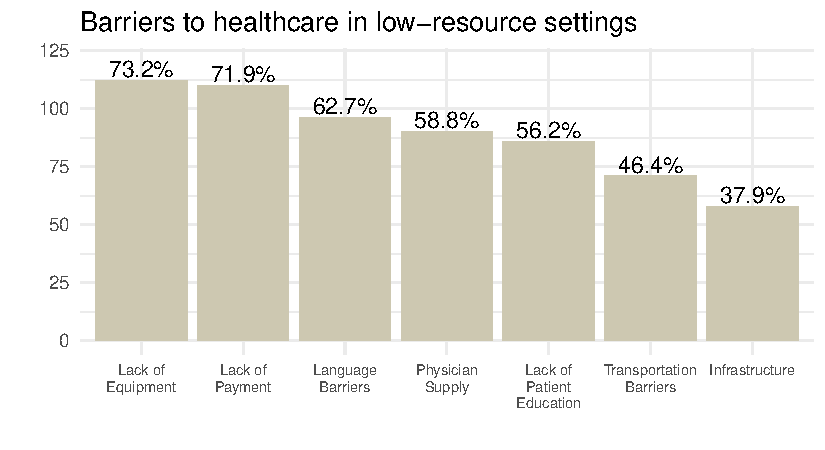
\includegraphics{GlobalHealthQuarto11-15_files/figure-pdf/unnamed-chunk-2-1.pdf}

\newpage

B. Barriers to Providing Healthcare by Global Health Career Interest

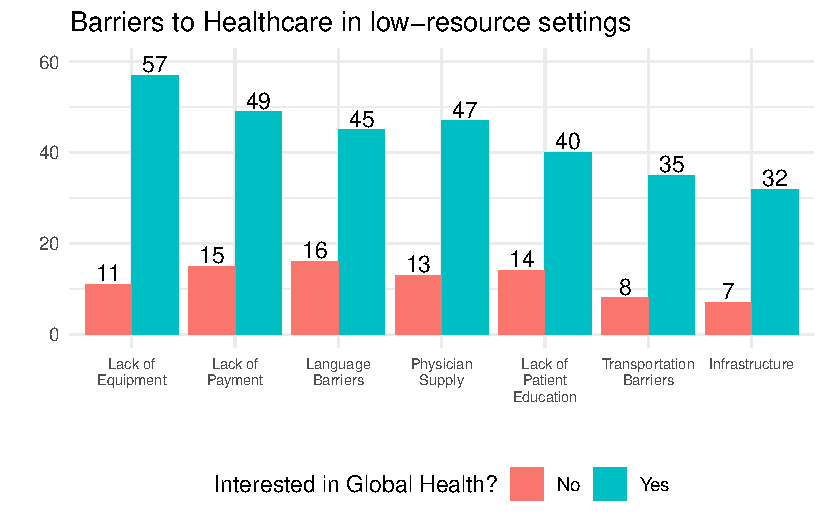
\includegraphics{GlobalHealthQuarto11-15_files/figure-pdf/unnamed-chunk-3-1.pdf}

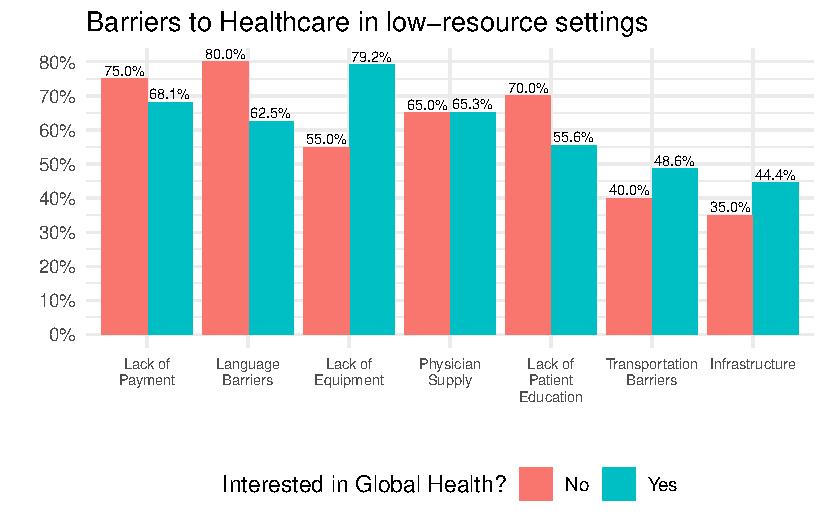
\includegraphics{GlobalHealthQuarto11-15_files/figure-pdf/unnamed-chunk-4-1.pdf}

\newpage

Below is a Chi Squared Test. This tests to see if the two distributions
of perceived barriers to low-resource healthcare are distinct from one
another. The test cannot confirm that there is a distinction. In other
words, the overall difference in perceived barriers to healthcare in low
resource settings of those who are interested in a Global Health Career
and those who are uninterested is not significant.

\begin{verbatim}
# 
#   Pearson's Chi-squared test
# 
# data:  df23gIntChi$Yes and df23gIntChi$No
# X-squared = 42, df = 36, p-value = 0.227
\end{verbatim}

\newpage

C. Barriers to Providing Healthcare by Born Abroad

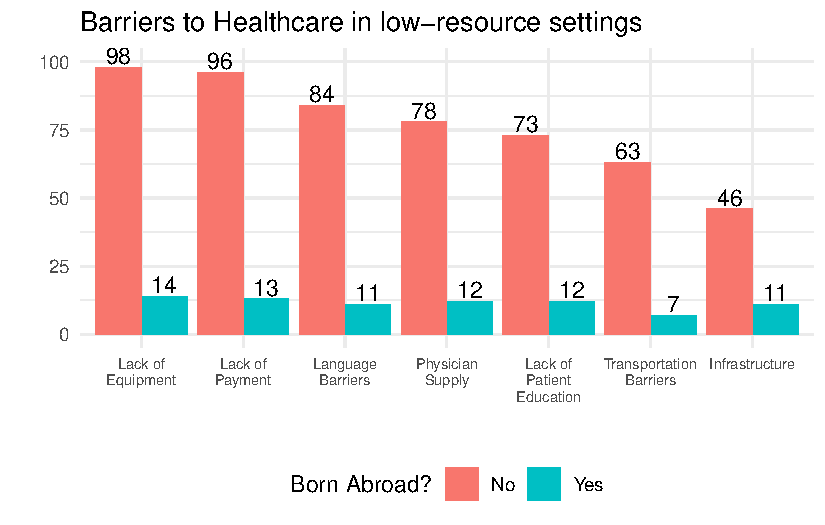
\includegraphics{GlobalHealthQuarto11-15_files/figure-pdf/unnamed-chunk-6-1.pdf}

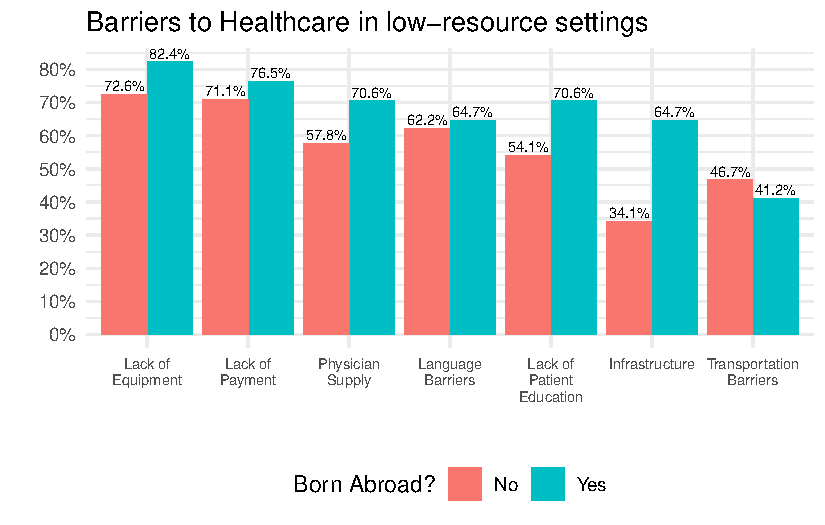
\includegraphics{GlobalHealthQuarto11-15_files/figure-pdf/unnamed-chunk-7-1.pdf}

\newpage

Below is a Chi Squared Test. This tests to see if the two distributions
of perceived barriers to low-resource healthcare are distinct from one
another. The test cannot confirm that there is a distinction. In other
words, the overall difference in perceived barriers to healthcare in low
resource settings of those who are interested in a Global Health Career
and those who are uninterested is not significant.

\begin{verbatim}
# 
#   Pearson's Chi-squared test
# 
# data:  df23gBornChi$Yes and df23gBornChi$No
# X-squared = 28, df = 24, p-value = 0.26
\end{verbatim}

\newpage

D. Barriers to Providing Healthcare by Lived Abroad

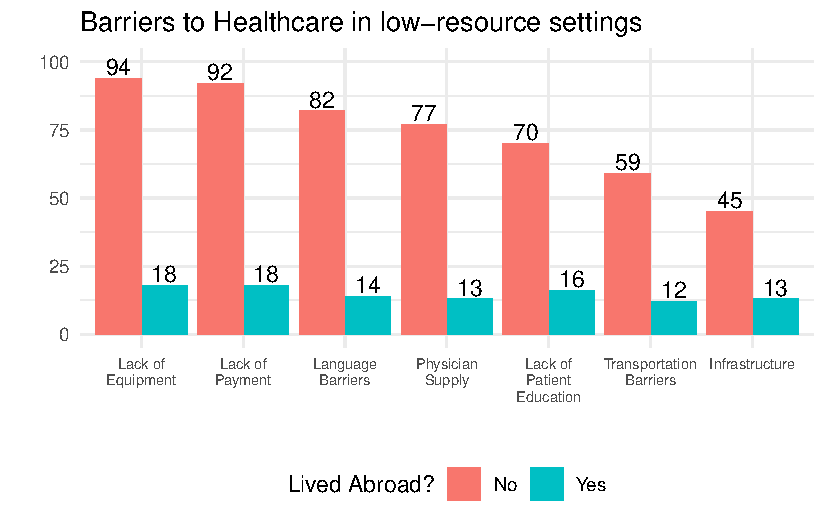
\includegraphics{GlobalHealthQuarto11-15_files/figure-pdf/unnamed-chunk-9-1.pdf}

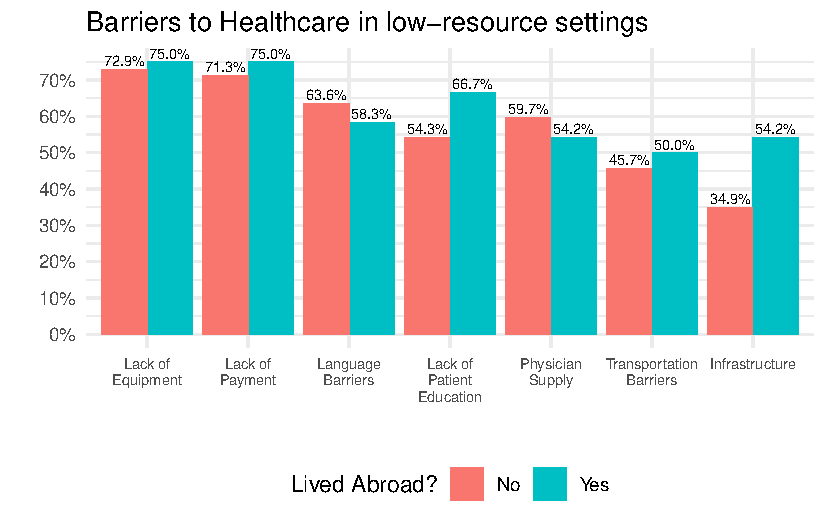
\includegraphics{GlobalHealthQuarto11-15_files/figure-pdf/unnamed-chunk-10-1.pdf}

\newpage

Below is a Chi Squared Test. This tests to see if the two distributions
of perceived barriers to low-resource healthcare are distinct from one
another. The test cannot confirm that there is a distinction. In other
words, the overall difference in perceived barriers to healthcare in low
resource settings of those who are interested in a Global Health Career
and those who are uninterested is not significant.

\begin{verbatim}
# 
#   Pearson's Chi-squared test
# 
# data:  df23gLivedChi$Yes and df23gLivedChi$No
# X-squared = 28, df = 24, p-value = 0.26
\end{verbatim}

\newpage

\hypertarget{rank-the-following-in-order-of-the-medical-field-that-you-believe-has-historically-had-the-greatest-impact-on-the-global-health-field-to-the-medical-field-you-believe-has-historically-had-the-least-impact-on-the-global-health-field.}{%
\subsection{12. Rank the following in order of the medical field that
you believe has historically had the GREATEST impact on the global
health field to the medical field you believe has historically had the
LEAST impact on the global health
field.}\label{rank-the-following-in-order-of-the-medical-field-that-you-believe-has-historically-had-the-greatest-impact-on-the-global-health-field-to-the-medical-field-you-believe-has-historically-had-the-least-impact-on-the-global-health-field.}}

\begin{verbatim}
# # A tibble: 11 x 6
#    Fields              Minimum `Q-1`  Mean `Q-3` Maximum
#    <chr>                 <dbl> <dbl> <dbl> <dbl>   <dbl>
#  1 Infectious Diseases       1     1  2.24     3      11
#  2 Emergency medicine        1     1  2.92     4      11
#  3 Family medicine           1     2  3.88     5      11
#  4 OB/GYN                    1     3  4.85     6      11
#  5 Surgical care             1     3  4.90     6      11
#  6 Pediatrics                1     4  5.29     6      11
#  7 Neurology                 2     6  7.56     9      11
#  8 Oncology                  2     7  7.65     9      11
#  9 Orthopedics               4     8  8.83    10      11
# 10 Psychiatry                2     8  8.89    11      11
# 11 Ophthalmology             3     8  8.98    10      11
\end{verbatim}

\newpage

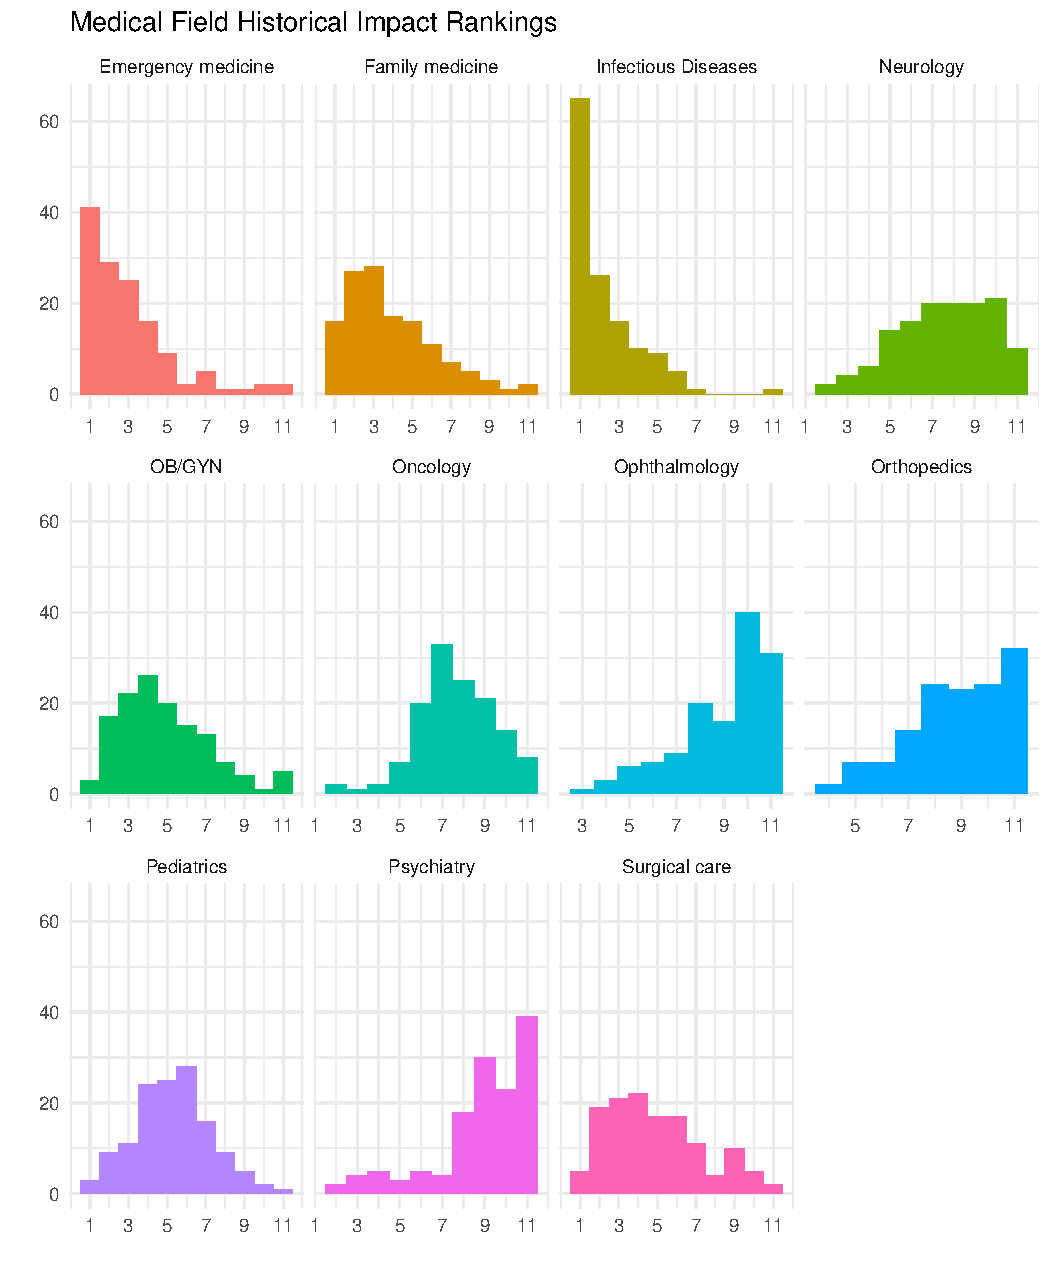
\includegraphics{GlobalHealthQuarto11-15_files/figure-pdf/unnamed-chunk-13-1.pdf}

\newpage

\hypertarget{rank-the-following-in-order-of-the-medical-field-that-you-believe-will-have-the-greatest-impact-on-the-global-health-field-in-the-future-to-the-medical-field-you-believe-will-have-the-least-impact-on-the-global-health-field-in-the-future.}{%
\subsection{13. Rank the following in order of the medical field that
you believe will have the GREATEST impact on the global health field in
the future to the medical field you believe will have the LEAST impact
on the global health field in the
future.}\label{rank-the-following-in-order-of-the-medical-field-that-you-believe-will-have-the-greatest-impact-on-the-global-health-field-in-the-future-to-the-medical-field-you-believe-will-have-the-least-impact-on-the-global-health-field-in-the-future.}}

\begin{verbatim}
# # A tibble: 11 x 6
#    Fields              Minimum `Q-1`  Mean `Q-3` Maximum
#    <chr>                 <dbl> <dbl> <dbl> <dbl>   <dbl>
#  1 Infectious Diseases       1     1  2.66     4      11
#  2 Emergency medicine        1     2  3.44     5      11
#  3 Family medicine           1     2  4.13     6      11
#  4 OB/GYN                    1     3  4.68     6      11
#  5 Surgical care             1     3  5.21     7      11
#  6 Pediatrics                1     4  5.70     8      10
#  7 Oncology                  1     6  7.02     9      11
#  8 Neurology                 1     6  7.14     9      11
#  9 Psychiatry                1     6  7.54     9      11
# 10 Orthopedics               1     8  9.19    11      11
# 11 Ophthalmology             2     9  9.28    11      11
\end{verbatim}

\newpage

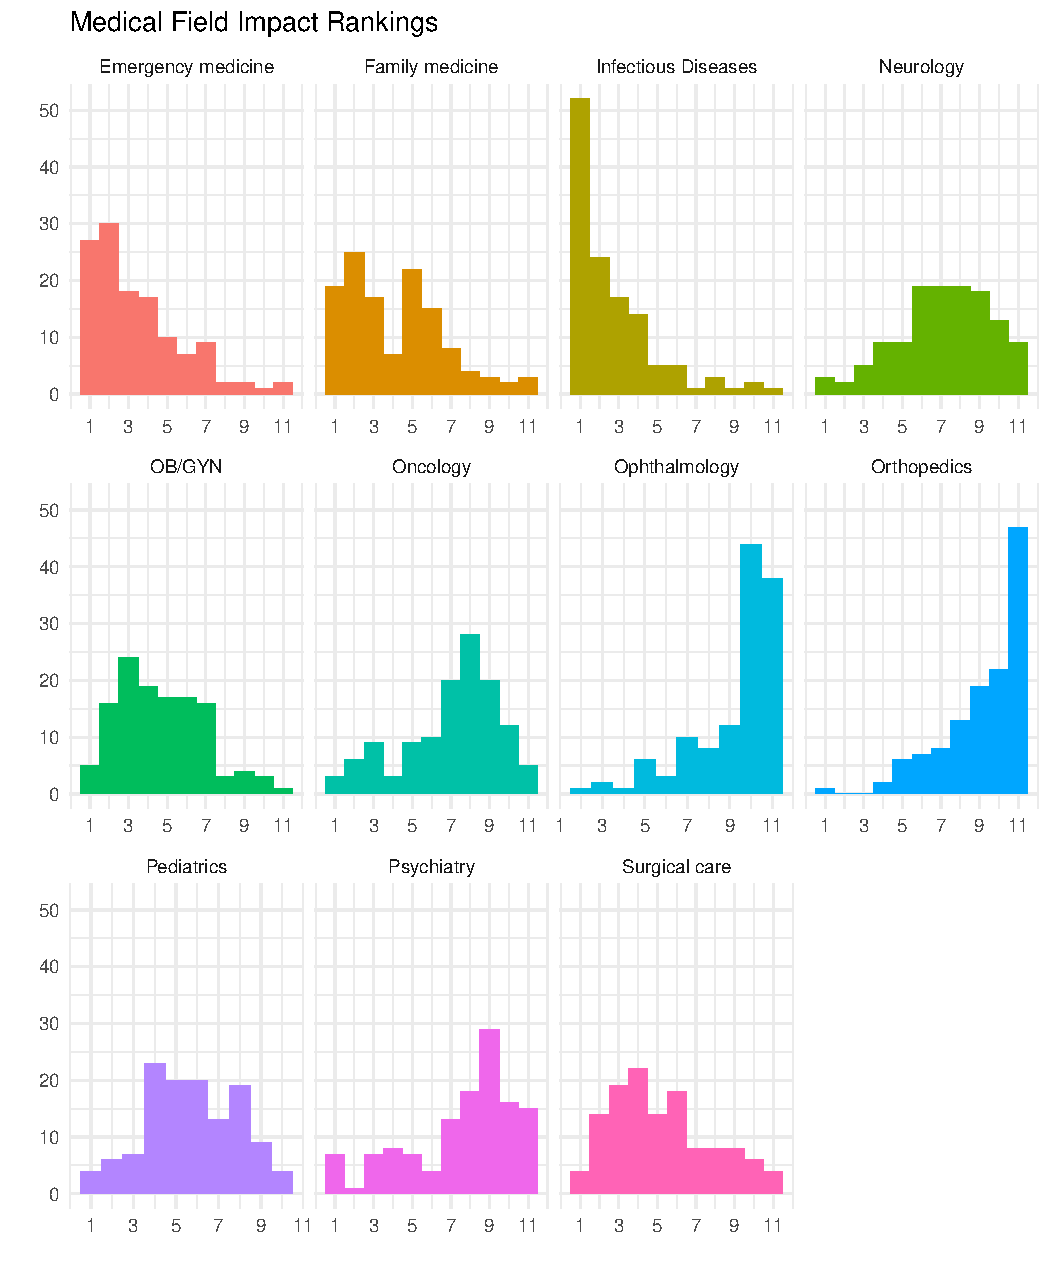
\includegraphics{GlobalHealthQuarto11-15_files/figure-pdf/unnamed-chunk-15-1.pdf}

\newpage

\hypertarget{in-your-opinion-which-three-of-the-following-medical-fields-contribute-most-to-strengthening-the-delivery-of-all-other-types-of-care}{%
\subsection{14. In your opinion, which THREE of the following medical
fields contribute MOST to strengthening the delivery of all other types
of
care?}\label{in-your-opinion-which-three-of-the-following-medical-fields-contribute-most-to-strengthening-the-delivery-of-all-other-types-of-care}}

A. Overall Results for Contribution of Various Medical Fields to other
types

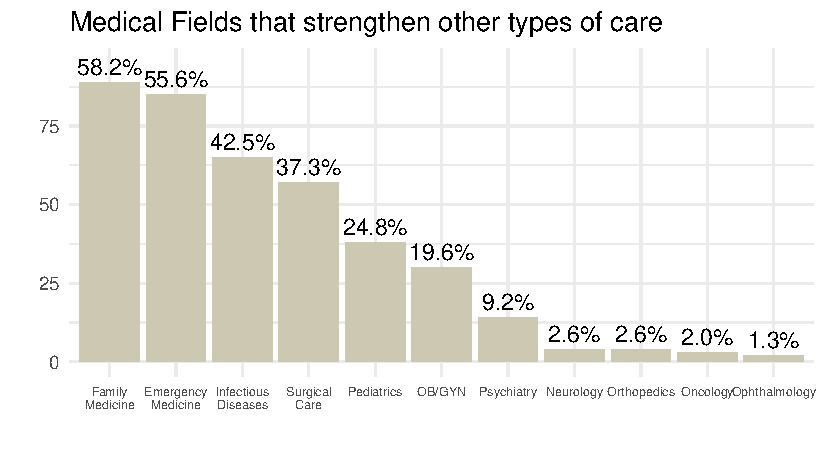
\includegraphics{GlobalHealthQuarto11-15_files/figure-pdf/unnamed-chunk-16-1.pdf}

\newpage

\hypertarget{increasing-access-to-surgical-care-should-be-a-priority-for-countries-increasing-access-to-healthcare.}{%
\subsection{15. Increasing access to surgical care should be a priority
for countries increasing access to
healthcare.}\label{increasing-access-to-surgical-care-should-be-a-priority-for-countries-increasing-access-to-healthcare.}}

A. Overall Results

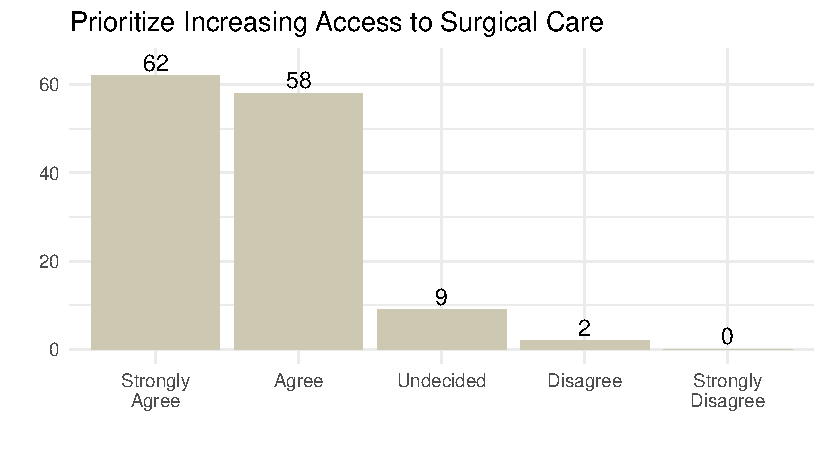
\includegraphics{GlobalHealthQuarto11-15_files/figure-pdf/unnamed-chunk-17-1.pdf}



\end{document}
